\documentclass[a4paper,10pt]{article}
\usepackage{wrapfig}
\usepackage{graphicx}

\title{6.829 Computer Networks\\Problem set 2}
\author{Shalev Ben-David, Yonatan Belinkov}

\begin{document}
\maketitle

\section{Measurements}
Figure~\ref{fig:fixedWindow} shows the performance of a protocol with a fixed window size. 
The best score we were able to achieve was -4.5 log(Throughput/Delay) with a window 
size of 15. However, the measurements were not very stable and varied by as much 
as 0.1 between different runs with the same window size. 

\begin{figure}[h]
 \begin{center}
  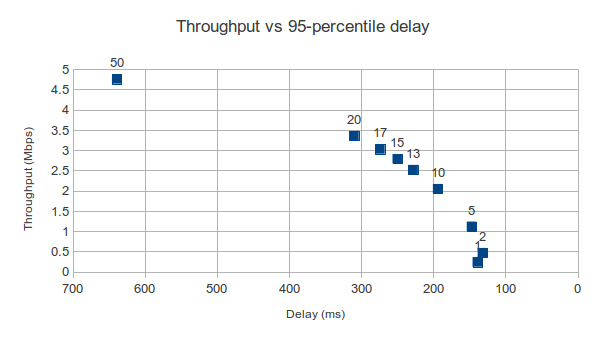
\includegraphics[width=1\textwidth]{fixedWindow.png}
  \end{center}
 \caption{Throughput vs 95-percentile delay with a fixed window size}
 \label{fig:fixedWindow}
\end{figure}

Our first try to implement an AIMD scheme did not produce very good results; we got
-5.84 log(Throughput/Delay) when adding $ 1/w $ to the window size on
every ACK and dividing by 2 on every timeout (timeout set to 1000 ms). A slower 
increase of $ 1/w^2 $ improved the score to -4.72. Another approach we tried was to
change the timeout, where we found out that decreasing the timeout to 100 ms improves
the score to -5.28 (while maintaining the standard AIMD). By combining both approaches
we managed to improve the score up to -4.12, by using a timeout of 100 ms, an additive 
increase of $ 1/w^2 $ on every ACK, and a harsher decrease of $ w \leftarrow \sqrt w $ 
on every timeout.

The delay-triggered scheme proved to be competitive with AIMD. We experimented with 
changing the window size based on when the RTT crosses a given threshold. 
Table~\ref{tab:delayTriggered} summarizes the results. The best score of -4.16 was achieved with a threshold 
of 100 ms, an increase of 0.1,\footnote{A non-integer increase effectively means 
that the window size changes only when it reaches the following integer} and a 
decrease of 1.

\begin{table}[h]
 \centering
 \begin{tabular}{|l|l|l|l|p{2cm}|l|}
 \hline
   Threshold (ms) & Increase & Decrease & Delay (ms) & Throughput (Mbps) & Score \\
 \hline
  100 & 1 & 1 & 308 & 3.39 & -4.51 \\
  200 & 1 & 1 & 580 & 4.02 & -4.97 \\
  50  & 1 & 1 & 162 & 1.75 & -4.53 \\
  100 & 2 & 2 & 436 & 3.76 & -4.75 \\
  100 & 1 & 2 & 299 & 3.12 & -4.56 \\
  100 & 0.1 & 1 & 155 & 2.41 & -4.16 \\
  \hline
 \end{tabular}
 \caption{Delay, throughput, and log(Throughput/Delay) score with different 
 delay-triggered schemes.}
 \label{tab:delayTriggered}
\end{table}


\end{document}